%%%% Document type  %%%%
\documentclass[preprint,12pt,fleqn]{article}
 \usepackage{ragged2e}
\usepackage{authblk}  % Package for author affiliations
% \usepackage{nopageno} % no page numbers
\usepackage{placeins} % \FloatBarrier

\usepackage[most]{tcolorbox}
\newtcolorbox[auto counter,number within=chapter]{definition}[1][]{
  enhanced,
  breakable,
  fonttitle=\scshape,
  title={Definition \thetcbcounter},
  #1
}

%%%% Document structure %%%%
%\usepackage{geometry}
\usepackage[verbose=true,letterpaper]{geometry}
\geometry{
%    a4paper,
%    left=30mm,
%    right=30mm,
%    top=30mm,
%    bottom=30mm,
    textheight=9in,
    textwidth=6in,
    top=1in,
    headheight=12pt,
    headsep=25pt,
    footskip=30pt,
   % phone  
   %a5paper,
   %width=120mm,
  %height=180mm,
}

\usepackage{lineno} % used along with \linenumbers after begin document. 
\usepackage{setspace} 
% \setstretch{1.4}
\makeatletter % The following lines get rid of footer stating pre-preint to elsevier.
\def\ps@pprintTitle{%
\let\@oddhead\@empty
\let\@evenhead\@empty
\def\@oddfoot{}%
\let\@evenfoot\@oddfoot}
\makeatother
\graphicspath{ {../images/} }
\usepackage{pgf} % calculate cohort stats percentage

%%%% Bibliography   %%%%
\usepackage{natbib}
\setcitestyle{numbers,sort&compress}
\setcitestyle{sort&compress}
\usepackage{hypernat} 
    
%%%% Aesthetics     %%%%
\usepackage{microtype}
% \RequirePackage{times} % Font
\usepackage{ccaption}
\usepackage{siunitx}
\usepackage[T1]{fontenc}
\usepackage[utf8]{inputenc}
\usepackage{nameref}% this allows a reference be named, to print unnumbered references by their section name (used here for linking to Supplemental text in this case).

%%%% Paragraph Formatting %%%
\setlength{\parindent}{0pt}
\setlength{\parskip}{6pt plus 2pt minus 1pt}

%%%% Supplemental labels%%%%
%Define command to start a supplemental section
%set the supplemental letter used for figures (e.g. Figure E1)
\newcommand{\beginsupplement}{%
        \setcounter{table}{0}
        \renewcommand{\thetable}{S\arabic{table}}%
        \setcounter{figure}{0}
        \renewcommand{\thefigure}{S\arabic{figure}}%
         }

%%%% Building tables%%%%
\usepackage{booktabs} % required for tables
\usepackage{rotating,tabularx} 
\newcolumntype{Z}{ >{\centering\arraybackslash}X } % defining table content layout per box
\usepackage{ltablex} % allow page break between lines in tabularx
% \usepackage{caption} \captionsetup{font=normalsize} % to set the caption size as normal even when table is tiny.
\usepackage{multirow}
\usepackage{pdflscape}

%%%% Colors %%%%
\usepackage{xcolor} 
\definecolor{natureblue}{RGB}{5,110,210}
    \usepackage[colorlinks]{hyperref} 
\AtBeginDocument{%this allows colours to chage from the defined elsearticle template.
\hypersetup{
    	colorlinks=true,
        linkcolor={natureblue},
    	citecolor={natureblue},
        filecolor=blue!50!black,
        urlcolor=cyan,
    	}}

\definecolor{kispiblack}{HTML}{333333}
\definecolor{kispidarkblue}{HTML}{023047}
\definecolor{kispidarkgreen}{HTML}{006666}
\definecolor{kispired}{HTML}{C70000}
\definecolor{kispilink}{HTML}{007DB8}%219EBC
% \color{kispi_black} %default
\definecolor{kispiblue}{HTML}{701A57}
% City sunset: https://www.color-hex.com/color-palette/40131
\definecolor{colorSUNSET1}{HTML}{eeaf61}
\definecolor{colorSUNSET2}{HTML}{fb9062}
\definecolor{colorSUNSET3}{HTML}{ee5d6c}
\definecolor{colorSUNSET4}{HTML}{ce4993}
\definecolor{colorSUNSET5}{HTML}{6a0d83}
\definecolor{natureblue}{RGB}{5,110,210}    
\usepackage{dirtree}  % Load the dirtree package


% command to use these colors and formatting; xspace for correct spacing including with punctuation marks.
\usepackage{xspace}
\newcommand{\variablesdarkgreen}[1]{\textbf{\textcolor{kispidarkgreen}{#1}}\xspace}

%%%% Fancy stuff %%%%
%\usepackage{fancyhdr}
%\pagestyle{fancy}
%\lhead{My Name}
%\chead{}
%\rhead{\thepage}
%\cfoot{} % get rid of the page number 
%\renewcommand{\headrulewidth}{0pt}
%\renewcommand{\footrulewidth}{0pt}
 
 
%\usepackage{fancyhdr}
%\usepackage{lastpage}
%\pagestyle{fancy}
%\fancyhf{}
%\rfoot{\thepage}
%\cfoot{} % get rid of the page number 
%\renewcommand{\headrulewidth}{0pt}
%\renewcommand{\footrulewidth}{0pt}

 
\usepackage{tocloft}  % Customizing the Table of Contents
\setcounter{tocdepth}{2}


%%%% Include code %%%%
% \usepackage{verbatim}

\usepackage{listings}
\lstset{
    basicstyle=\ttfamily\small,
    breaklines=true,
    postbreak=\mbox{\textcolor{red}{$\hookrightarrow$}\space}, % 
    breakatwhitespace=false,
    % frame=single,
    showstringspaces=TRUE, % Don't show spaces in strings as special characters
    tabsize=2, 
    language=sh 
}

\usepackage{fontspec}
% \setmainfont{IBM Plex Sans}
% \setmonofont{IBM Plex Mono}
% \usepackage{unicode-math}
% \setmathfont{IBM Plex Math}

%\renewcommand{\rmdefault}{ptm}
%\renewcommand{\sfdefault}{phv}


% {{\ttfamily \hyphenchar\the\font=`\-} % set hyphenation for texttt blocks









% nips 2017 settings


\begin{document}
\title{PanelAppRex: A Sophisticated Search Function for Gene Panel Data}	
\author[1]{Dylan Lawless\thanks{Addresses for correspondence: \href{mailto:Dylan.Lawless@uzh.ch}{Dylan.Lawless@uzh.ch}}}

\affil[1]{Department of Intensive Care and Neonatology, University Children's Hospital Zürich, University of Zürich, Switzerland.}


\maketitle
\justify


\maketitle

\begin{abstract}
\noindent
\textbf{Motivation:} Gene panel data provides critical insights into disease-gene correlations. However, aggregating and interrogating this diverse dataset can be challenging. PanelAppRex addresses this by first preparing a machine-readable aggregate and second by offering a sophisticated natural language search interface that streamlines data exploration for both clinical and research applications.\\[1ex]
\textbf{Results:} PanelAppRex aggregates gene panel data from source including CliVar, Uniprot, and Genomics England’s PanelApp, including the approved panels used in the NHS National Genomic Test Directory and the 100,000 Genomes Project. It enables users to execute complex queries by gene names, phenotypes, disease groups and more, returning integrated datasets in multiple downloadable formats. Benchmarking demonstrates that the system effectively simplifies variant discovery and interpretation to enhance workflow efficiency. The greatest benefit is the analysis ready format for bioinformatic integration.\\[1ex]
\textbf{Availability and implementation:} PanelAppRex is available under the MIT licence. The source code and data are accessible at \url{https://github.com/DylanLawless/PanelAppRex}. The dataset is maintained for a minimum of two years following publication.
\end{abstract}

\section{Introduction}
\noindent
Gene panels are pivotal for the diagnosis and interpretation of genetic disorders. Sources like Genomics England’s PanelApp and PanelApp Australia host comprehensive panels that support genomic testing \cite{martin_panelapp_2019}. For instance, these are integral in the NHS and research projects such as the 100,000 Genomes Project. Despite its utility, manual panel selection and data aggregation remain labour intensive. PanelAppRex was developed to simplify this process by automating data retrieval from the PanelApp API and integrating the data into machine and user-friendly formats. The novel natural language search capability further streamlines the discovery of disease gene panels by allowing queries based on gene names, phenotypes, disease groups and additional key attributes which were generated with evidence-based Retrieval-augmented generation (RAG).


\section{Materials and methods}
\subsection{Implementation}
\noindent
PanelAppRex is implemented in R and integrates data from Genomics England’s PanelApp. It performed credentialed access to the API to retrieve all approved panels, merging them into two formats: a simplified version (Panel ID, Gene) and a complex version (including metadata such as confidence level, mode of inheritance, and disease information), and several metadata summary statistics. In addition, the tool incorporates a natural language processing module to interpret and execute complex user queries. The search functionality supports queries by gene names, phenotypes, disease names, disease groups, panel names, genomic locations and other identifiers. 
RAG was used to improve the natural queries in hidden states based on evidence about the disease and gene function by supplementing the data with additional sources including ClinVar, UniProt, etc. 

\subsection{Usage}
\noindent
Online, queries can be executed via the integrated search bar in our HTML version, where a JavaScript function splits the query into individual terms and progressively filters rows - retaining only those that match all active terms while ignoring unmatched ones. This enables users to perform complex, partial matching queries (e.g. ``paediatric RAG1 primary immunodeficiency skin disorder'') to rapidly identify the panel most closely associated with their hypothesis on primary immunodeficiency and paediatric skin disorders.

Bioinformatically, users can import the provided, ready-for-use, datasets in TSV or Rds formats. Users are most likely to merge with their own omic data based on merging with gene/protein ID.
The following code snippet, available in \texttt{minimal\_example.R}, demonstrates how to load the data in R:
\begin{verbatim}
# TSV format
path_data <- "../data"
core_path <- paste0(path_data, "/PanelAppData_combined_core")
minimal_path <- paste0(path_data, "/PanelAppData_combined_minimal")

df_core <- read.table(
    file= paste0(core_path, ".tsv"), 
    sep = "\t", header = TRUE)

df_minimal <- read.table(
    file= paste0(minimal_path, ".tsv"), 
    sep = "\t", header = TRUE)

# Rds format
rds_path <- paste0(path_data, "/PanelAppData_combined_Rds")
df_core <- readRDS(file= rds_path)
\end{verbatim}


\section{Results}
\noindent
PanelAppRex successfully aggregates data, currently from 451 panels, and several genomics databases to offer a user-friendly natural language search functionality (\textbf{Figure \ref{fig:performance}}).
Users can retrieve results filtered by gene names, phenotypes, disease groups and other criteria. The system returns a table view with panel details and provides options for exporting results in CSV, Excel, or PDF formats.

\begin{figure}[ht]
    \centering
    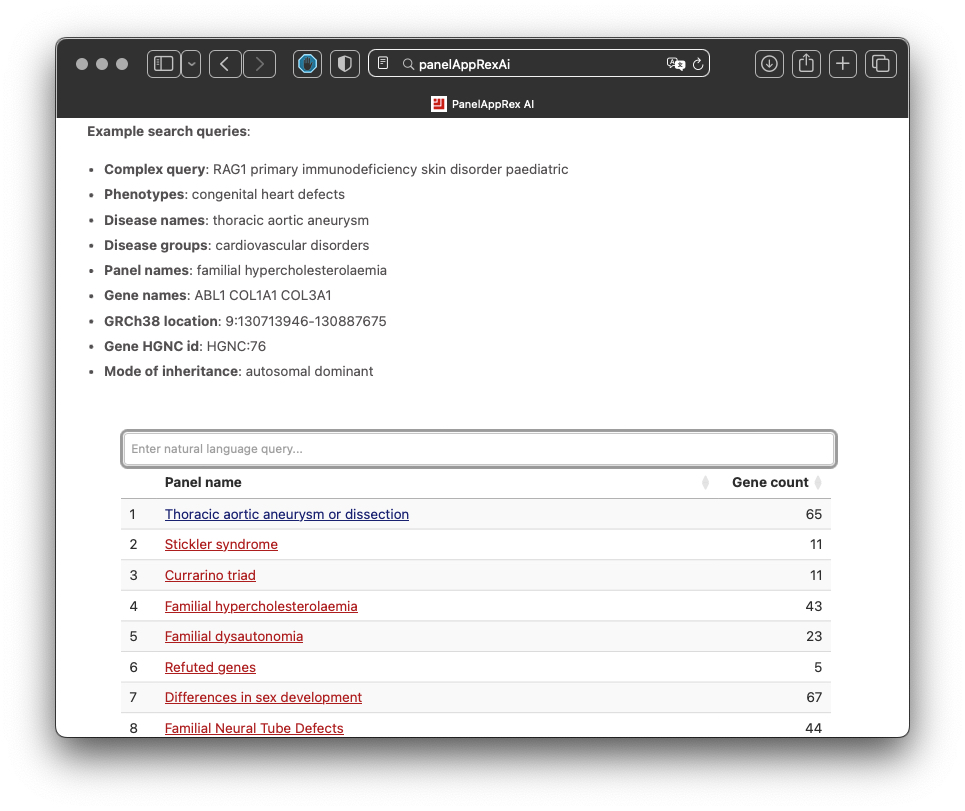
\includegraphics[width=0.49\textwidth]{screenshot_1.jpg}
    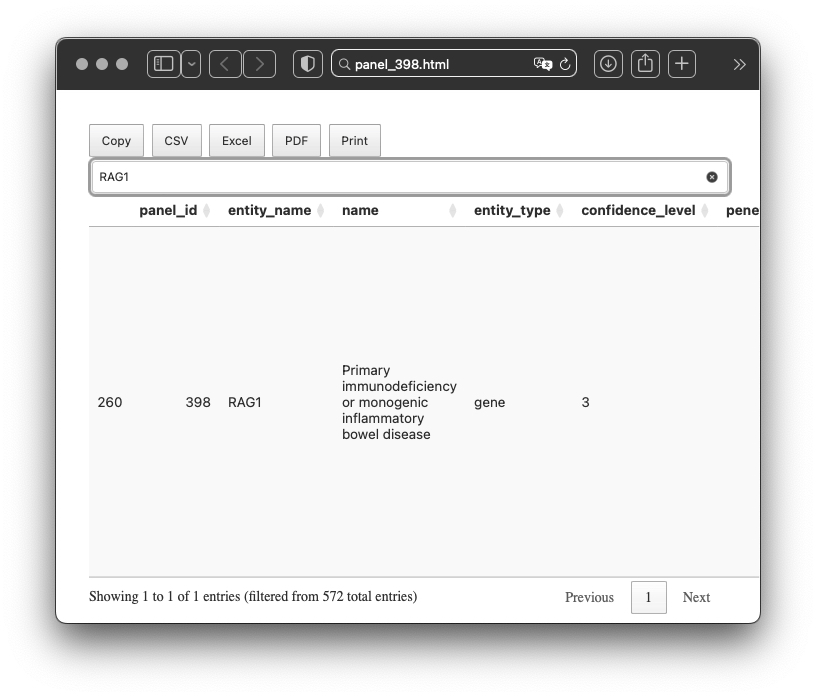
\includegraphics[width=0.49\textwidth]{screenshot_2.jpg}    
    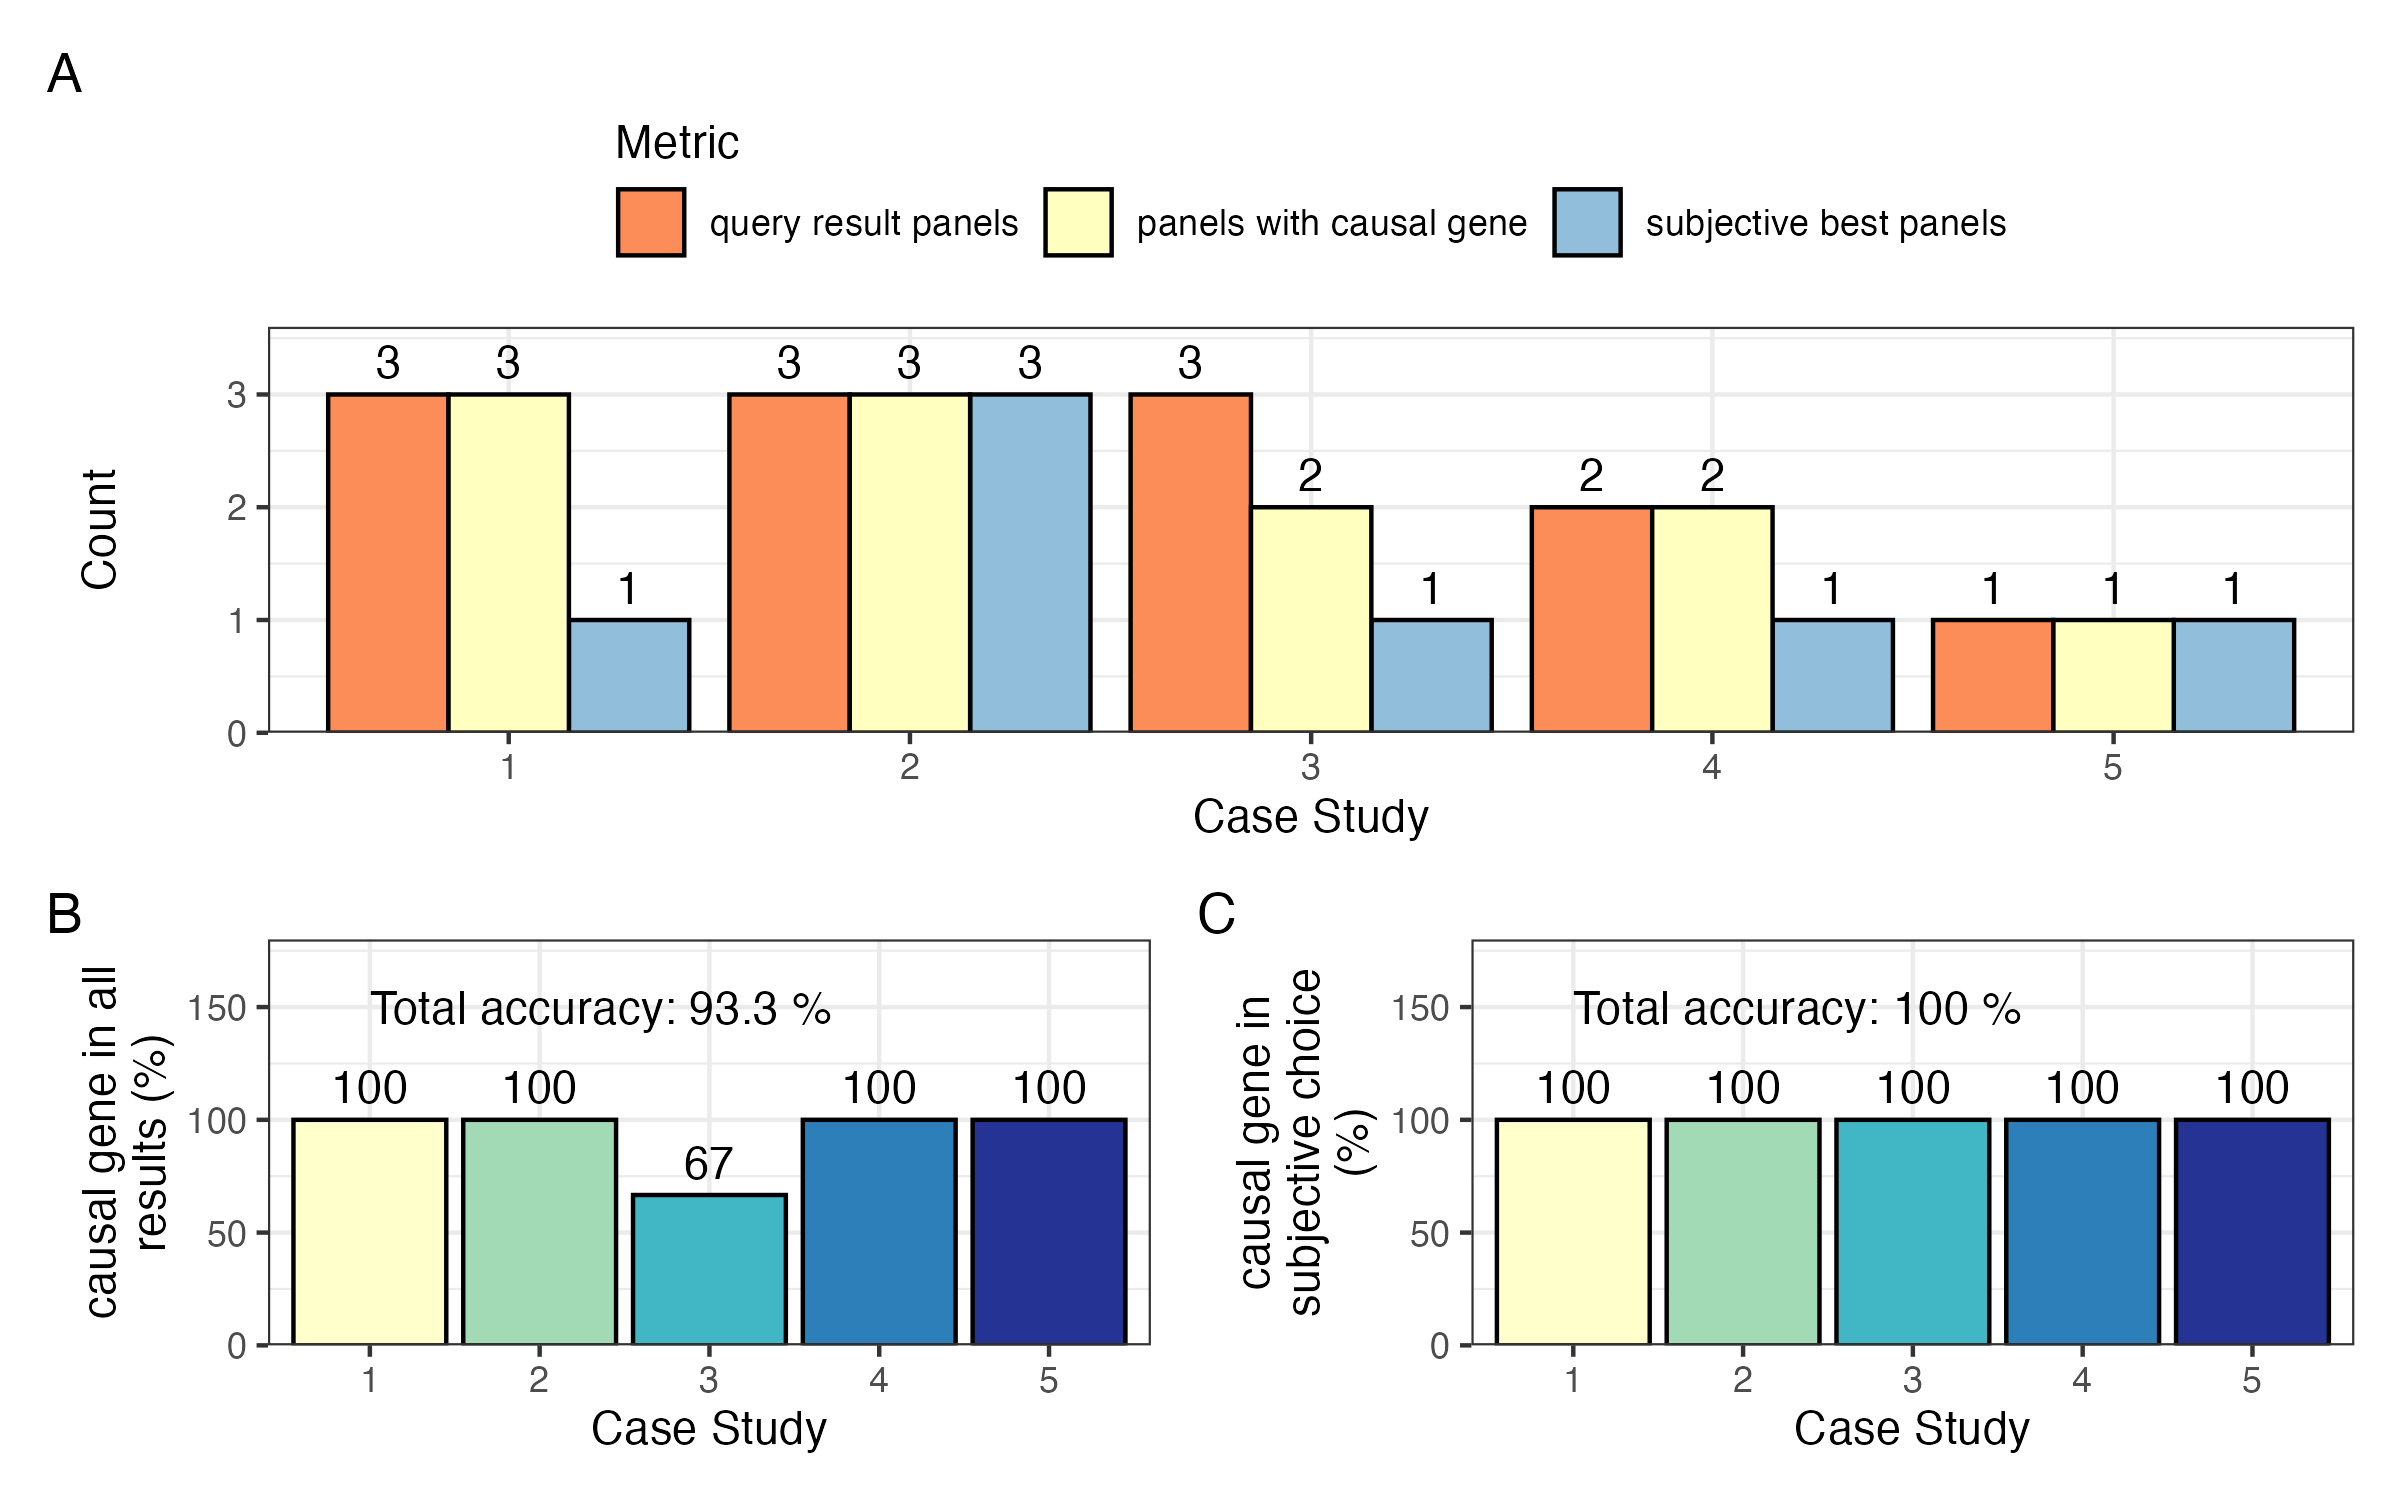
\includegraphics[width=0.75\textwidth]{benchmark.png}    
    \caption{Screenshot of the PanelAppRex interface displaying search results for a complex natural language query. Key metrics such as panel name and gene count are displayed in a user-friendly table format. The left window shows the whole database before searching for a panel. The right window shows the result of selecting a panel, revealing the complete detailed data table.}
    \label{fig:performance}
\end{figure}

\subsection{Validation benchmarking}
\noindent
To mimic a clinician diagnosing a new disease such as primary immunodeficiency (PID), we began by systematically selecting from the current online catalogue from the Journal of Allergy and Clinical Immunology (JACI), using the first five results  \cite{arruda_genetic_2015, 
mcaleer_severe_2015,
verhoeven_hematopoietic_2022,
magerus-chatinet_autoimmune_2013,
sharfe_fatal_2014}. The clinical background from these studies was used to construct keyword queries from patient features, simulating a naïve starting position for a clinician (full sources, queries, and results in supplemental table 1). We then tested whether our PanelAppRex tool could successfully retrieve panels that included the final causal gene reported in each case study. 

In our evaluation, PanelAppRex returned panels in which the causal gene was present in 93\% of all cases, with the user-selected best panel achieving a perfect accuracy of 100\% 
(\textbf{Figure \ref{fig:performance}}).
 These metrics were derived by comparing the causal gene identified from the case study abstracts to the panels returned by our query, and by applying a subjective relevance measure to mimic intuitive panel selection - acknowledging that certain panels, such as the established PID gene panel, are inherently more reliable than broader, less specific panels. Overall, the results confirm that our approach accurately identifies the most relevant panels and effectively supports clinical decision-making in complex diagnostic scenarios.


\FloatBarrier
\section{Summary}
\noindent
PanelAppRex offers a robust solution for aggregating and querying gene panel data. Its sophisticated natural language search feature simplifies data exploration and enhances variant interpretation. Future work will focus on expanding the range of supported queries and integrating additional genomic data sources, further supporting the needs of clinicians and researchers.

\section*{Acknowledgements}
\noindent
We acknowledge Genomics England for providing public access to the PanelApp data.
The use of data from Genomics England panelapp was licensed under the Apache License 2.0 A permissive license whose main conditions require preservation of copyright and license notices. Contributors provide an express grant of patent rights. Licensed works, modifications, and larger works may be distributed under different terms and without source code. These permissions consist of commercial use, modification, distribution, patent use, and  private use.

\bibliographystyle{unsrtnat}
\bibliography{references.bib}
\clearpage

\end{document}